\documentclass{lehramt-informatik}
\InformatikPakete{syntax,mathe}
\usepackage{tikz}
\usepackage{pifont}
\usepackage{multicol}
\usepackage{blkarray}
\usetikzlibrary{petri,arrows.meta}

\def\TmpSetKeys{%
  \def\TmpTransitionOne{}%
  \def\TmpTransitionTwo{}%
  \def\TmpTransitionThree{}%
  \def\TmpTransitionFour{}%
  \def\TmpTransitionFive{}%
  \def\TmpTransitionSix{}%
  \def\TmpTransitionSeven{}%
  \def\TmpTransitionEight{}%
  \def\TmpTransitionNine{}%
  \def\TmpTransitionTen{}%
  \pgfkeys{/petri/.cd,
    p1/.store in=\TmpPlaceOne,p1/.default=0,p1,
    p2/.store in=\TmpPlaceTwo,p2/.default=0,p2,
    p3/.store in=\TmpPlaceThree,p3/.default=0,p3,
    p4/.store in=\TmpPlaceFour,p4/.default=0,p4,
    p5/.store in=\TmpPlaceFive,p5/.default=0,p5,
    p6/.store in=\TmpPlaceSix,p6/.default=0,p6,
    p7/.store in=\TmpPlaceSeven,p7/.default=0,p7,
    p8/.store in=\TmpPlaceEight,p8/.default=0,p8,
    p9/.store in=\TmpPlaceNine,p9/.default=0,p9,
    p10/.store in=\TmpPlaceTen,p10/.default=0,p10,
    t1/.store in=\TmpTransitionOne,t1/.default=activated,
    t2/.store in=\TmpTransitionTwo,t2/.default=activated,
    t3/.store in=\TmpTransitionThree,t3/.default=activated,
    t4/.store in=\TmpTransitionFour,t4/.default=activated,
    t5/.store in=\TmpTransitionFive,t5/.default=activated,
    t6/.store in=\TmpTransitionSix,t6/.default=activated,
    t7/.store in=\TmpTransitionSeven,t7/.default=activated,
    t8/.store in=\TmpTransitionEight,t8/.default=activated,
    t9/.store in=\TmpTransitionNine,t9/.default=activated,
    t10/.store in=\TmpTransitionTen,t10/.default=activated,
    scale/.store in=\TmpScale,scale/.default=0.5,
    x/.store in=\TmpX,x/.default=5,
    y/.store in=\TmpY,y/.default=5,
  }%
}

\TmpSetKeys

\tikzset{activated/.style={very thick}}

\begin{document}

%%%%%%%%%%%%%%%%%%%%%%%%%%%%%%%%%%%%%%%%%%%%%%%%%%%%%%%%%%%%%%%%%%%%%%%%
% Theorie-Teil
%%%%%%%%%%%%%%%%%%%%%%%%%%%%%%%%%%%%%%%%%%%%%%%%%%%%%%%%%%%%%%%%%%%%%%%%

\chapter{Petri-Netze}

\section{Simulatoren}

\begin{itemize}
\item \url{http://petri.hp102.ru/pnet.html} (online)
\item \url{https://apo.adrian-jagusch.de/} (online)
\item \url{https://www.oris-tool.org/}
\item \url{https://github.com/sarahtattersall/PIPE}
\end{itemize}

\def\TmpBeschriftung#1{%
  {%
    \footnotesize%
    \itshape#1%
  }%
}

\noindent
Petri-Netze stellen einen Formalismus zur Beschreibung
\memph{nebenläufiger Ereignisse} dar.
%
Sie können somit u.\,a. \memph{zur Planung eines Softwareprojektes}
genutzt werden.
\footcite{sosy:fs:3}

\begin{description}

%%
%
%%

\item[Stellen/Platz (place)] Eine Stelle wird mit einem Kreis
%
(\tikz
\node[place,minimum size=7pt]{};)
%
dargestellt.

\begin{description}
\item[Kapazität]
Jedem Platz wird als „Schranke“ eine natürliche Zahl zugeordnet. Wenn
beim Eintritt einer Transition mehr als in der Kapazitäts-Schranke
angegeben Marken auf dem Platz entstehen würden, ist die Transition
nicht aktiviert.
\footcite{wiki:petri-netz}

\bigskip
\centerline{\fbox{\tikz \node[place,label=1,label=south:\TmpBeschriftung{Kapazität 1}]{};
\tikz \node[place,label=3,label=south:\TmpBeschriftung{Kapazität 3}]{};
\tikz \node[place,label=5,label=south:\TmpBeschriftung{Kapazität 5}]{};}}

\item[Belegung] Belegung nennt man die Anzahl der Tokens auf einem
Platz. Standardmäßig sind Plätze nicht belegt, d.\,h. sie haben keine
Tokens und damit die Belegung 0. Anstatt den kleinen Kreisen kann auch
eine Zahl in die Plätzen eintragen werden. Die Zahl steht dann für die
Anzahl der Tokens.

\bigskip
\centerline{\fbox{
  \tikz \node[place,label=south:\TmpBeschriftung{Belegung 0}]{};
  \tikz \node[place,tokens=1,label=south:\TmpBeschriftung{Belegung 1}]{};
  \tikz \node[place,tokens=3,label=south:\TmpBeschriftung{Belegung 3}]{};
  \tikz \node[place,tokens=5,label=south:\TmpBeschriftung{Belegung 5}]{};
  \tikz \node[place,label=south:\TmpBeschriftung{Belegung 7}]{7};
}}
\end{description}

%%
%
%%

\item[Transition/Schaltstelle (transition)]
Eine Transition wird mit einem Viereck
%
(\tikz[scale=0.5,transform shape] \node[transition]{};)
%
dargestellt. Anstelle des Rechtecks sind auch Striche
%
(\tikz
\node[rectangle,fill=black,minimum width=0.5mm,minimum height=2mm,inner
sep=0pt]{};)
%
gebräuchlich. Eine Transition kann nur schalten, wenn sich
im Eingang ein Token gefindet.

Eine Transition kann feuern (schalten), wenn jede Eingangsstelle mit
mindestens so vielen Token belegt ist, wie das Gewicht des zugehörigen
Pfeils angibt und wenn in jeder Ausgangsstelle die Zahl der vorhandenen
Marken plus dem Gewicht des zugehörigen Pfeils die Kapazität nicht
übersteigt.
\footcite[Seite 9]{sosy:fs:3}

%%
%
%%

\item[Kante/Pfeil (arc)]

Die Knoten sind durch gerichtete Kanten
%
(\tikz \draw[->] (0,0) -- (0.5,0);)
%
verbunden, wobei eine Kante genau eine Stelle mit einer Transition oder
umgekehrt verbindet. Die Kanten dürfen jeweils nur von Stellen zu
Transitionen oder von Transitionen zu Stellen führen.
\footnote{\url{https://kroening-online.de/Method/Petrinetz/m_petri.php}}

\textbf{erlaubt:}

\begin{center}
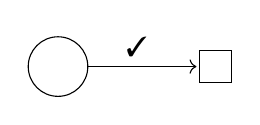
\begin{tikzpicture}
\node[place](p) {};
\node[transition] at (2,0) {} edge[pre] (p);
\node at (1,0.25) {\ding{51}};
\end{tikzpicture}
%
\hspace{1cm}
%
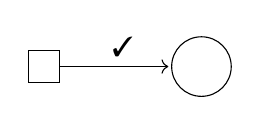
\begin{tikzpicture}
\node[place] at (2,0) (p) {};
\node[transition] at (0,0) {} edge[post] (p);
\node at (1,0.25) {\ding{51}};
\end{tikzpicture}
\end{center}

\textbf{nicht erlaubt:}

\begin{center}
\raisebox{5pt}{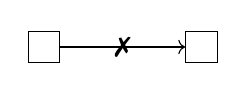
\begin{tikzpicture}
\node[transition] at (0,0) (t1) {};
\node[transition] at (2,0) (t2) {};
\draw[->] (t1) -- (t2);
\node at (1,0) {\ding{55}};
\end{tikzpicture}}
%
\hspace{1cm}
%
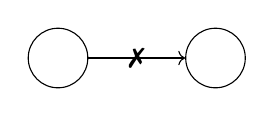
\begin{tikzpicture}
\node[place] at (0,0) (p1) {};
\node[place] at (2,0) (p2) {};
\draw[->] (p1) -- (p2);
\node at (1,0) {\ding{55}};
\end{tikzpicture}
\end{center}

\begin{description}
\item[Gewichtung]
Durch eine \emph{Gewichtung} der Kanten kann die \emph{Anzahl der
Marken} angegeben werden, die entnommen bzw. erzeugt werden.
\footnote{\url{http://ddi.cs.uni-potsdam.de/HyFISCH/Produzieren/SeminarDidaktik/Nebenlaeufigkeit/marken.htm}}
Die Gewichtung wird durch Ganzezahlen in der Mitte des Pfeils notiert.

\begin{center}
\def\TmpGewichtung#1{\tikz \draw[->] (0,0) -- (1.5,0) node[pos=0.5,auto]{\scriptsize#1};}
\TmpGewichtung{}
\TmpGewichtung{3}
\TmpGewichtung{5}
\end{center}
\end{description}

\item[Marke/Markierung (token)] Die Kennzeichnung der Belegung einer
Stelle wird durch einen kleinen ausgefüllten Kreis gezeichnet (\tikz
\node[token]{};).

\item[„Inhibitor“-Kante (inhibitor arc)]
Anstelle der Pfeilspitze wird bei der Inhibitor-Kante an Kreis gezeichnet
(\tikz \draw[-{Circle[open,length=2mm,fill=white]}] (0,0) -- (1,0);).
Einen Platz auf Abwesenheit von
Marken testen: Ein Platz $p$ ist mit einer Transition $t$ durch eine
„Inhibitor“-Kante verbunden. $t$ ist nicht aktiviert, wenn $p$
eine oder mehrere Marken trägt.
\footcite{wiki:petri-netz}

\def\TmpInhibitor#1{
  \begin{tikzpicture}[x=1.5cm,y=0.8cm]
    \node[place,tokens=1,label=$p_1$] at (0,2) (A) {};
    \node[place,tokens=#1,label=$p_2$] at (0,0) (B) {};
    \node[place,label=$p_3$] at (2,1) (C) {};
    \node[transition] at (1,1) (t) {$t$}
      edge[pre] (A)
      edge[post] (C)
    ;

    \draw[-{Circle[open,length=2mm,fill=white]}] (B) -- (t);
  \end{tikzpicture}
}

\begin{multicols}{2}
$t$ ist nicht aktiviert:\\
\TmpInhibitor{1}

$t$ ist aktiviert:\\
\TmpInhibitor{0}
\end{multicols}

\end{description}

%-----------------------------------------------------------------------
%
%-----------------------------------------------------------------------

\section{Darstellungsmatrix}

Ein Petri-Netz kann mit einer Matrix dargestellt werden.
Vorgängerstellen werden mit negativem Vorzeichen in der Spalte der
Transition eingetragen. Die Nachfolger mit positivem. Ein  Vektor gibt
die Anfangsmarkierung an.
\footnote{\url{https://www.hs-augsburg.de/informatik/projekte/mebib/emiel/entw_inf/lernprogramme/petrinetze/NetzAnalyse1HTML.html}}
%-----------------------------------------------------------------------
%
%-----------------------------------------------------------------------

\section{Begriffe\footcite[Seite 10]{sosy:fs:3}}

\begin{description}
\item[Verklemmung]
Ein Petri-Netz heißt \emph{verklemmungsfrei}, wenn keine Verklemmung
erreichbar ist. Eine Verklemmung (= Deadlock) ist ein Zustand, in dem
keine einzige Transition schalten kann.

\begin{multicols}{2}
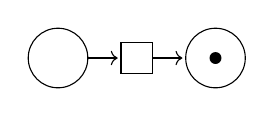
\begin{tikzpicture}
\node[place] at (0,0) (p1)  {};
\node[place,tokens=1] at (2,0) (p2) {};
\node[transition] at (1,0) {} edge[pre] (p1) edge[post] (p2);
\end{tikzpicture}

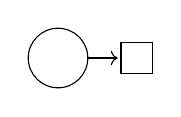
\begin{tikzpicture}
\node[place] at (0,0) (p1)  {};
\node[transition] at (1,0) {} edge[pre] (p1);
\end{tikzpicture}
\footnote{\url{https://www.is.inf.uni-due.de/courses/mod_ws14/folien/petri-print.pdf}}
\end{multicols}

\item[Lebendigkeit (Transition)]
Eine Transition heißt \emph{lebendig}, wenn es für jeden möglichen
Zustand endlich viele Schaltvorgänge gibt, so dass diese Transition
schalten kann.

\item[Lebendigkeit (Petri-Netz)]
Ein Petri-Netz heißt \emph{lebendig}, wenn alle Transitionen lebendig
sind. Insbesondere ist jedes lebendige Petri-Netz verklemmungsfrei.

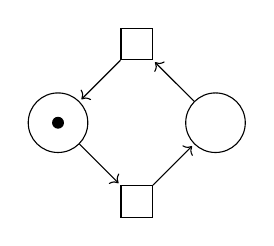
\begin{tikzpicture}
\node[place,tokens=1] at (0,0) (p1)  {};
\node[place] at (2,0) (p2) {};
\node[transition] at (1,1) {} edge[pre] (p2) edge[post] (p1);
\node[transition] at (1,-1) {} edge[pre] (p1) edge[post] (p2);
\end{tikzpicture}
\footnote{\url{https://www.is.inf.uni-due.de/courses/mod_ws14/folien/petri-print.pdf}}

\begin{description}
\item[Starke Lebendigkeit]
Starke Lebendigkeit bedeutet, dass es \emph{überall} im System immer
wieder zu Schaltungen kommen kann.

\item[Schwache Lebendigkeit]
Bei schwacher Lebendigkeit kann es immer wieder \emph{irgendwo} zu
Schaltungen kommen.
\footnote{\url{http://wwwlgis.informatik.uni-kl.de/cms/fileadmin/courses/ss2007/Informationssysteme/Kapitel.09.Petrinetze.full.pdf}}

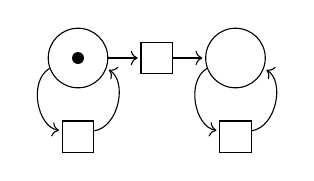
\begin{tikzpicture}
\node[place,tokens=1] at (0,1) (p1)  {};

\node[place] at (2,1) (p2) {};

\node[transition] at (0,0) {} edge[pre,bend left=70] (p1) edge[post,bend right=70] (p1);

\node[transition] at (1,1) {} edge[pre] (p1) edge[post] (p2);

\node[transition] at (2,0) {} edge[pre,bend left=70] (p2) edge[post,bend right=70] (p2);
\end{tikzpicture}
\footnote{\url{http://www.ti.inf.uni-due.de/fileadmin/public/teaching/mod/slides/ws201112/petri-2x2.pdf}}

\end{description}

\item[Beschränktheit]
Ein Petri-Netz heißt \emph{beschränkt}, wenn es eine Konstante $1$ gibt,
so dass jede Stelle zu jedem möglichen Zustand höchstens $M$ Marken
enthält.

\item[Umkehrbarkeit]
Ein Petri-Netz heißt \emph{umkehrbar}, wenn die Anfangsmarkierung von
jeder erreichbaren Markierung erreichbar ist. Das Petri-Netz ist nicht
umkehrbar, wenn es verklemmt ist.
\end{description}

\section{Beispiele für Schaltungen}

Die Zustandsänderung erfolgt durch das Schalten der Transition, aber nur
wenn \emph{alle} Stellen des Vorbereichs  markiert sind. Dann wird in
\emph{jeder} Stelle des Nachbereichs eine Marke erzeugt.
\footnote{\url{http://ddi.cs.uni-potsdam.de/HyFISCH/Produzieren/SeminarDidaktik/Nebenlaeufigkeit/marken.htm}}

\def\TmpSchaltungEins#1#2#3#4#5{
  \begin{tikzpicture}
  \node[place,tokens=#1] at (0,0.5) (p1) {};
  \node[place,tokens=#2] at (0,-0.5) (p2) {};

  \node[place,tokens=#3] at (4,1) (p3) {};
  \node[place,tokens=#4] at (4,0) (p4) {};
  \node[place,tokens=#5] at (4,-1) (p5) {};

  \node[transition] at (2,0) {}
    edge[pre] (p1)
    edge[post] (p3)
    edge[pre] (p2)
    edge[post] (p4)
    edge[post] (p5)
  ;
  \end{tikzpicture}
}

\begin{multicols}{2}
vorher:

\TmpSchaltungEins{1}{2}{1}{0}{0}

nachher:

\TmpSchaltungEins{0}{1}{2}{1}{1}
\end{multicols}

%%
%
%%

\noindent
Eine Transition kann hier nur Schalten, wenn die Anzahl der Marken
mindestens der Gewichtung im Vorbereich entspricht bzw. die
Gewichtung im Nachbereich nicht überschritten wird.
\footnote{\url{http://ddi.cs.uni-potsdam.de/HyFISCH/Produzieren/SeminarDidaktik/Nebenlaeufigkeit/marken.htm}}

\def\TmpSchaltungZwei#1#2#3#4{
  \medskip
  \begin{tikzpicture}
    \node[place,tokens=#1] at (0,2) (p1) {};
    \node[place,tokens=#2] at (0,0) (p2) {};

    \node[place,tokens=#3] at (4,2) (p3) {};
    \node[place,tokens=#4] at (4,0) (p4) {};

    \node[transition] at (2,1) {}
      edge[pre] (p1)
      edge[pre] node[auto] {2} (p2)

      edge[post] node[auto] {3} (p3)
      edge[post] (p4)
    ;
  \end{tikzpicture}
}

\begin{multicols}{2}
vorher:

\TmpSchaltungZwei{2}{2}{0}{0}

\columnbreak

nachher:

\TmpSchaltungZwei{1}{0}{3}{1}
\end{multicols}

%%
%
%%

\def\TmpSchaltungDrei#1#2#3#4{
  \medskip
  \begin{tikzpicture}
    \node[place,tokens=#1,label=$s_1$] at (0,2) (p1) {};
    \node[place,tokens=#2,label=$s_2$] at (0,0) (p2) {};

    \node[place,tokens=#3,label=$s_3$] at (4,2) (p3) {};
    \node[place,tokens=#4,label=$s_4$] at (4,0) (p4) {};

    \node[transition] at (2,1) {t}
      edge[pre] node[auto] {2} (p1)
      edge[pre] node[auto] {1} (p2)

      edge[post] node[auto] {1} (p3)
      edge[post] node[auto] {3} (p4)
    ;
  \end{tikzpicture}
}

\begin{multicols}{2}
vorher:\footcite[Seite 9 (von Wikipedia)]{sosy:fs:3}

\TmpSchaltungDrei{3}{1}{1}{0}

\columnbreak

nachher:

\TmpSchaltungDrei{1}{0}{2}{3}
\end{multicols}

%-----------------------------------------------------------------------
%
%-----------------------------------------------------------------------

\section{Erreichbarkeitsgraph
\footcite[Seite 11]{sosy:fs:3}}

Ein Erreichbarkeitsgraph (auch Markierungsgraph genannt) ist ein
gerichteter Graph, der aus einem Petri-Netz und einer Anfangsmarkierung
gewonnen werden kann. Er wird dadurch erzeugt, dass, mit der
Anfangsmarkierung beginnend, die Menge der in der Markierung aktivierten
Transitionen ermittelt und jeweils die Folgemarkierung berechnet wird.
Die Markierungen werden durch Knoten im Erreichbarkeitsgraphen
dargestellt und der Übergang einer Markierung zu ihrer Folgemarkierung
wird als Kante im Graphen vermerkt. Für jede Folgemarkierung wird dieser
Vorgang wiederholt.\footcite{wiki:erreichbarkeitsgraph}

\def\TmpErreichbar(#1,#2,#3,#4)#5{
\begin{tikzpicture}[scale=#5,transform shape]
    \node[place,label=$s_1$,tokens=#1] at (0,1.5) (s1) {};
    \node[place,label=$s_2$,tokens=#2] at (3,1.5) (s2) {};
    \node[place,label=$s_3$,tokens=#3] at (0,0)   (s3) {};
    \node[place,label=$s_4$,tokens=#4] at (3,0)   (s4) {};

    \node[transition] at (1.5,1.5) {$t_1$}
      edge[pre] (s1)
      edge[post] (s2);
    \node[transition] at (1.5,0) {$t_2$}
      edge[pre] (s3)
      edge[post] (s4);
    \node[transition] at (4.5,0.75) {$t_3$}
      edge[pre] (s2)
      edge[pre] (s4)
      edge[post,bend right=70] (s1)
      edge[post,bend left=70] (s3);
  \end{tikzpicture}
}

\bigskip
\ueberschrift{Beispiel} Gegeben sie folgendes Petri-Netz:

\begin{center}
\TmpErreichbar(2,0,1,0){1}
\end{center}

\bigskip
\ueberschrift{Ergebnis} Daraus ergibt sich folgender Erreichbarkeitsgraph:

\begin{center}
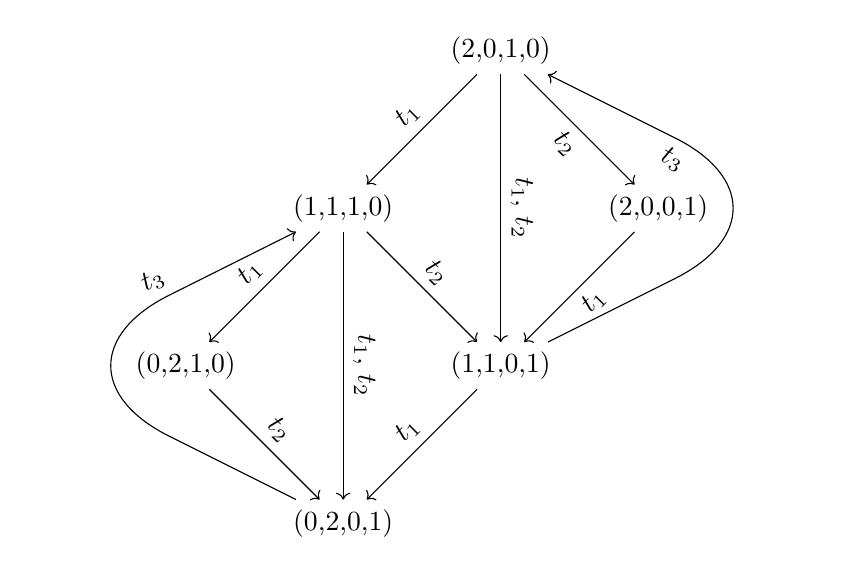
\begin{tikzpicture}[x=2cm,y=2cm]
\def\pfeil#1#2#3#4{\draw[->] (#1) -- (#2) node[pos=0.5,auto,sloped,#4]{#3};}
\node at (2,3) (2010) {(2,0,1,0)};
\node at (1,2) (1110) {(1,1,1,0)};
\node at (3,2) (2001) {(2,0,0,1)};
\node at (0,1) (0210) {(0,2,1,0)};
\node at (2,1) (1101) {(1,1,0,1)};
\node at (1,0) (0201) {(0,2,0,1)};

\pfeil{2010}{1110}{$t_1$}{}
\pfeil{2010}{1101}{$t_1$, $t_2$}{}
\pfeil{2010}{2001}{$t_2$}{swap}
\pfeil{1110}{0210}{$t_1$}{}
\pfeil{1110}{0201}{$t_1$, $t_2$}{}
\pfeil{1110}{1101}{$t_2$}{}
\pfeil{0210}{0201}{$t_2$}{}
\pfeil{1101}{0201}{$t_1$}{}
\pfeil{2001}{1101}{$t_1$}{swap}

\draw[->,rounded corners=2cm] (1101) -- (4,2) -- (2010) node[pos=0.5,sloped,auto,swap]{$t_3$};
\draw[->,rounded corners=2cm] (0201) -- (-1,1) -- (1110) node[pos=0.5,sloped,auto]{$t_3$};
\end{tikzpicture}
\end{center}

\begin{multicols}{5}
\noindent
(1,1,1,0):
\TmpErreichbar(1,1,1,0){0.4}

\noindent
(2,0,0,1):
\TmpErreichbar(2,0,0,1){0.4}

\noindent
(1,1,0,1):
\TmpErreichbar(1,1,0,1){0.4}

\noindent
(0,2,1,0):
\TmpErreichbar(0,2,1,0){0.4}

\noindent
(0,2,0,1):
\TmpErreichbar(0,2,0,1){0.4}
\end{multicols}

%%%%%%%%%%%%%%%%%%%%%%%%%%%%%%%%%%%%%%%%%%%%%%%%%%%%%%%%%%%%%%%%%%%%%%%%
% Aufgaben
%%%%%%%%%%%%%%%%%%%%%%%%%%%%%%%%%%%%%%%%%%%%%%%%%%%%%%%%%%%%%%%%%%%%%%%%

\chapter{Aufgaben}

\section{Aufgabe 2: „Petri-Netze“\footcite{sosy:pu:4}}

Gegeben sei das folgende Petri-Netz:\footcite[Seite 9]{examen:46116:2016:03}

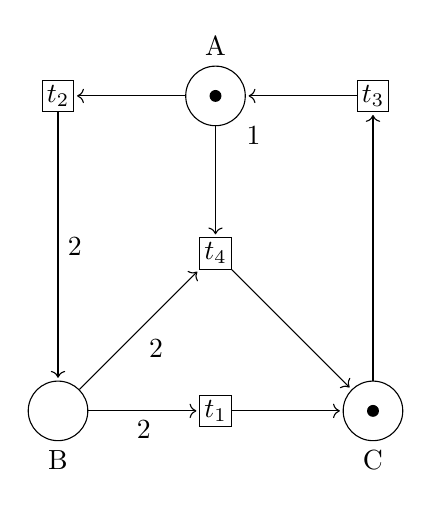
\begin{tikzpicture}[x=2cm,y=2cm]
  \node[place,label=A,label=south east:1,tokens=1] at (1,2) (A) {};
  \node[place,label=south:B] at (0,0) (B) {};
  \node[place,label=south:C,tokens=1] at (2,0) (C) {};

  \node[transition] at (1,0) {$t_1$}
    edge[pre] node[auto]{2} (B)
    edge[post] (C);

  \node[transition] at (0,2) {$t_2$}
    edge[pre] (A)
    edge[post] node[auto]{2} (B);

  \node[transition] at (2,2) {$t_3$}
    edge[pre] (C)
    edge[post] (A);

  \node[transition] at (1,1) {$t_4$}
    edge[pre] (A)
    edge[pre] node[auto]{2} (B)
    edge[post] (C);

\end{tikzpicture}

\begin{enumerate}

%%
% a)
%%

\item Erstellen Sie den zum Petri-Netz gehörenden
Erreichbarkeitsgraphen. Die Belegungen sind jeweils in der Form [A, B,
C] anzugeben. Beschriften Sie auch jede Kante mit der zugehörigen
Transition. Beachten Sie die auf 1 beschränkte Kapazität von Stelle A
oder alternativ die Inhibitor-Kante von A zu t3 (beides ist hier
semantisch äquivalent).

%%
% b)
%%

\item Wie kann man mit Hilfe des Erreichbarkeitsgraphen feststellen, ob
ein Petri-Netz lebendig ist?

%%
% c)
%%

\item Aufgrund von Transition t4 ist das gegebene Petri-Netz nicht stark
lebendig. Wie müssten die Pfeilgewichte der Transition t4 verändert
werden, damit das Petri-Netz mit der gegebenen Startmarkierung
beschränkt bleibt und lebendig wird?

\end{enumerate}

%-----------------------------------------------------------------------
%
%-----------------------------------------------------------------------

\section{Aufgabe 1: Begriffe\footcite[Seite 1]{sosy:ab:4}}

Begründen Sie, welche der folgenden Petri-Netze

%%
%
%%

\def\TmpA#1{
  \TmpSetKeys%
  \pgfkeys{/petri/.cd,#1}%
  \begin{tikzpicture}
  \node at (-0.25,-0.25) {};
  \node at (\TmpX,\TmpY) {};

  \begin{scope}[transform canvas={scale=\TmpScale},x=2cm,y=2cm,]
    \node[place,tokens=\TmpPlaceOne,label=$p_1$] at (0,1) (p1) {};
    \node[place,tokens=\TmpPlaceTwo,label=$p_2$] at (2,2) (p2) {};
    \node[place,tokens=\TmpPlaceThree,label=east:$p_3$] at (2,0) (p3) {};

    \node[transition,label=east:$t_1$,\TmpTransitionOne] at (2,1) {}
      edge[pre] (p2)
      edge[post] (p3);
    \node[transition,label=$t_2$,\TmpTransitionTwo] at (1,1.5) {}
      edge[pre] (p1)
      edge[post] (p2);
    \node[transition,label=$t_3$,\TmpTransitionThree] at (1,0.5) {}
      edge[pre] (p3)
      edge[post] (p1);
    \node[transition,label=$t_4$,\TmpTransitionFour] at (1,1) {}
      edge[pre] (p2)
      edge[pre] (p3)
      edge[post] (p1);
  \end{scope}
  \end{tikzpicture}
}

%%
%
%%

\def\TmpB#1{
  \TmpSetKeys%
  \pgfkeys{/petri/.cd,#1}%
  \begin{tikzpicture}
  \node at (-0.25,-0.25) {};
  \node at (\TmpX,\TmpY) {};

  \begin{scope}[transform canvas={scale=\TmpScale},x=2cm,y=2cm,]
    \node[place,tokens=\TmpPlaceOne,label=$p_1$] at (0,2) (p1) {};
    \node[place,tokens=\TmpPlaceTwo,label=$p_2$] at (0,0) (p2) {2019};
    \node[place,tokens=\TmpPlaceThree,label=east:$p_3$] at (2,1) (p3) {};

    \node[transition,label=east:$t_1$,\TmpTransitionOne] at (1,1.5) {}
      edge[pre] (p3)
      edge[post] (p1);
    \node[transition,label=$t_2$,\TmpTransitionTwo] at (1,1) {}
      edge[pre] (p1)
      edge[pre] (p2)
      edge[post] (p3);
    \node[transition,label=$t_3$,\TmpTransitionThree] at (1,0.5) {}
      edge[pre] (p2)
      edge[post] (p2)
      edge[post] (p3);
  \end{scope}
  \end{tikzpicture}
}

%%
%
%%

\def\TmpC#1{%
  \TmpSetKeys%
  \pgfkeys{/petri/.cd,#1}%
  \begin{tikzpicture}
    \node at (-0.25,-0.25) {};
    \node at (\TmpX,\TmpY) {};
    \begin{scope}[transform canvas={scale=\TmpScale},x=2cm,y=2cm,]
    \node[place,tokens=\TmpPlaceOne,label=west:$p_1$] at (0,4) (p1) {};
    \node[place,tokens=\TmpPlaceTwo,label=west:$p_2$] at (0,2) (p2) {};
    \node[place,tokens=\TmpPlaceThree,label=west:$p_3$] at (0,0) (p3) {};
    \node[place,tokens=\TmpPlaceFour,label=$p_4$] at (1,2) (p4) {};
    \node[place,tokens=\TmpPlaceFive,label=east:$p_5$] at (3,0) (p5) {};
    \node[place,tokens=\TmpPlaceSix,label=east:$p_6$] at (3,2) (p6) {};
    \node[place,tokens=\TmpPlaceSeven,label=east:$p_7$] at (3,4) (p7) {};

    \node[transition,label=west:$t_1$,\TmpTransitionOne] at (0,3) {}
      edge[pre] (p1)
      edge[post] node[auto] {2} (p2) edge[post] (p4);

    \node[transition,label=$t_2$,\TmpTransitionTwo] at (2,4) {}
      edge[pre] (p7)
      edge[post] (p1);

    \node[transition,label=south:$t_3$,\TmpTransitionThree] at (2,0) {}
      edge[pre] (p3)
      edge[post] (p5) edge[post] (p6);

    \node[transition,label=$t_4$,\TmpTransitionFour] at (2,2) {}
      edge[pre] node[auto] {2} (p6)
      edge[post] (p4);

    \node[transition,label=west:$t_5$,\TmpTransitionFive] at (0,1) {}
      edge[pre] (p2) edge[pre] (p4)
      edge[post] (p3);

    \node[transition,label=east:$t_6$,\TmpTransitionSix] at (3,1) {}
      edge[pre] (p5)
      edge[post] (p6);

    \node[transition,label=east:$t_7$,\TmpTransitionSeven] at (3,3) {}
      edge[pre] (p6)
      edge[post] (p7) edge[post] (p1);
    \end{scope}
  \end{tikzpicture}%
}

\def\TmpD#1{
  \TmpSetKeys%
  \pgfkeys{/petri/.cd,#1}%
  \begin{tikzpicture}
    \node at (-0.25,-0.25) {};
    \node at (\TmpX,\TmpY) {};
    \begin{scope}[transform canvas={scale=\TmpScale},x=2cm,y=2cm,]
    \node[place,tokens=\TmpPlaceOne,label=west:$p_1$] at (0,2) (p1) {};
    \node[place,tokens=\TmpPlaceTwo,label=$p_2$] at (2,2) (p2) {};
    \node[place,tokens=\TmpPlaceThree,label=$p_3$] at (4,2) (p3) {};
    \node[place,tokens=\TmpPlaceFour,label=east:$p_4$] at (6,2) (p4) {};
    \node[place,tokens=\TmpPlaceFive,label=east:$p_5$] at (6,0) (p5) {};
    \node[place,tokens=\TmpPlaceSix,label=$p_6$] at (4,0) (p6) {};
    \node[place,tokens=\TmpPlaceSeven,label=$p_7$] at (2,0) (p7) {};
    \node[place,tokens=\TmpPlaceEight,label=west:$p_8$] at (0,0) (p8) {};
    \node[place,tokens=\TmpPlaceNine,label=$p_9$] at (4,1) (p9) {};
    \node[place,tokens=\TmpPlaceTen,label=$p_{10}$] at (2,1) (p10) {};

    \node[transition,label=$t_1$,\TmpTransitionOne] at (1,2) {}
      edge[pre] (p1) edge[pre] (p10)
      edge[post] (p2);
    \node[transition,label=$t_2$,\TmpTransitionTwo] at (3,2) {}
      edge[pre] (p2) edge[pre] (p9)
      edge[post] (p10) edge[post] (p3);
    \node[transition,label=$t_3$,\TmpTransitionThree] at (5,2) {}
      edge[pre] (p3)
      edge[post] (p9) edge[post] (p4);
    \node[transition,label=east:$t_4$,\TmpTransitionFour] at (6,1) {}
      edge[pre] (p4)
      edge[post] (p5);
    \node[transition,label=$t_5$,\TmpTransitionFive] at (5,0) {}
      edge[pre] (p5) edge[pre] (p9)
      edge[post] (p6);
    \node[transition,label=$t_6$,\TmpTransitionSix] at (3,0) {}
      edge[pre] (p6) edge[pre] (p10)
      edge[post] (p7) edge[post] (p9);
    \node[transition,label=$t_7$,\TmpTransitionSeven] at (1,0) {}
      edge[pre] (p7)
      edge[post] (p10) edge[post] (p8);
    \node[transition,label=west:$t_8$,\TmpTransitionEight] at (0,1) {}
      edge[pre] (p8)
      edge[post] (p1);
    \end{scope}
  \end{tikzpicture}
}
\begin{enumerate}
\item beschränkt
\item lebendig
\item verklemmungsfrei
\item umkehrbar
\end{enumerate}

\begin{enumerate}
\item \TmpA{x=3.3,y=2.5,scale=0.7,p2=2}
\item \TmpB{x=3.3,y=2.5,scale=0.7}
\item \TmpC{x=3.3,y=5.5,scale=0.7,p1=1}
\item \TmpD{x=3.3,y=3,scale=0.7,p1=2,p5=2,p9=1,p10=1}

\end{enumerate}

\begin{antwort}

\ueberschrift{(a)}

\tikzset{/petri/.cd,x=2,y=2,scale=0.45}

\noindent
\TmpA{p2=2,t1,}
%
\TmpA{p2=1,p3=1,t1,t3,t4,}
%
\TmpA{p1=1,p3=1,t2,t3,}
%
\TmpA{p1=1,p2=1,t1,t2,}

\begin{description}
\item[beschränkt] ja, $M = 2$.

\item[lebendig] Nein, die Transition $t_4$ kann maximal einmal schalten
(z. B. $t_1 \rightarrow t_4$)

\item[verklemmungsfrei] Ja, mit $t_1 \rightarrow t_3 \rightarrow  t_2$
ist ein Zyklus gegeben.

\item[umkehrbar] Nein, nachdem $t_4$ einmal geschaltet hat, wird dem
Petri-Netz eine Markierung entzogen, welche nie wieder erzeugt werden
kann.
\end{description}

\ueberschrift{(b)}

\begin{description}
\item[beschränkt] Nein, solange in $p_2$ mindestens eine Markierung ist,
kann $t_3$ beliebig oft schalten und somit die Anzahl der Markierungen
in $p_3$ beliebig erhöhen.

\item[lebendig] Nein, da es nicht verklemmungsfrei ist.

\item[verklemmungsfrei] Nein, nachdem 2019 mal $t_2$ und anschließend
$t_1$ geschaltet haben, befindet sich in $p_2$ keine Marke mehr. Daher
können weder $t_2$ noch $t_3$ schalten.

\item[umkehrbar]
Nein, da es nicht verklemmungsfrei ist.
\end{description}

\ueberschrift{(c)}

\begin{description}
\item[beschränkt] Nein, $t_1 \rightarrow t_5 \rightarrow t_3 \rightarrow
t_6 \rightarrow t_7 \rightarrow t_2$ bildet einen Zyklus, der nach jedem
Umlauf die Anzahl der Marken in $p_1$ um eins erhöht.

\item[lebendig] Nein, da es nicht verklemmungsfrei ist.

\item[verklemmungsfrei] Nein, die Schaltfolge $t_1 \rightarrow t_5
\rightarrow t_3 \rightarrow t_6 \rightarrow t_4 \rightarrow t_5
\rightarrow t_3 \rightarrow t_6 \rightarrow t_4$ führt zu einer
Verklemmung.

\item[umkehrbar] Nein, da es nicht verklemmungsfrei ist.

\end{description}

\tikzset{/petri/.cd,x=3.3,y=4.3,scale=0.45}

\noindent
\TmpC{p1=1,t1}
\TmpC{p2=2,p4=1,t5}
\TmpC{p2=1,p3=1,t3}
\TmpC{p2=1,p5=1,p6=1,t4,t7,t6}
\TmpC{p1=1,p2=1,p7=1,p6=1,t1,t2,t4,t5,t7}
\TmpC{p1=2,p2=1,p7=1,t1,t2,t5,t7}

\ueberschrift{(d)}

\begin{description}
\item[beschränkt] Ja, mit M = 4.

\item[lebendig] Ja.

\item[verklemmungsfrei] Ja.

\item[umkehrbar] Ja.
\end{description}

\end{antwort}

\noindent
sind.
%
Im Falle der Beschränktheit soll ein minimales $M$ gefunden werden,
sodass jede Stelle zu jedem möglichen Zeitpunkt höchstens $M$ Marken
enthält.

%-----------------------------------------------------------------------
%
%-----------------------------------------------------------------------

\section{Aufgabe 2: Modellierung\footcite[Seite 2]{sosy:ab:4}}

Modellieren Sie folgendes Szenario als Petri-Netz:

Ein Modul gilt als bestanden, wenn beide Prüfungen $P_1$ und $P_2$
bestanden sind. Beide Prüfungen dürfen bei Nicht-Bestehen jeweils
maximal zwei mal wiederholt werden. Die Prüfungen dürfen nicht
gleichzeitig geschrieben werden. Erst wenn eine von beiden bestanden
wurde, darf die nächste begonnen werden. Wurde eine der beiden Prüfungen
insgesamt drei mal nicht bestanden, so gilt das gesamte Modul als nicht
bestanden.

%-----------------------------------------------------------------------
%
%-----------------------------------------------------------------------

\section{Aufgabe 3: Rechnen\footcite[Seite 2]{sosy:ab:4}}

Gegeben sei die Darstellungsmatrix $A$ und der Belegungsvektor $v$ eines
Petri-Netzes:

\begin{displaymath}
A =
\begin{blockarray}{ccccc}
  & t_1 & t_2 & t_3 & t_4 \\
  \begin{block}{c(cccc)}
  p_1 & -1 & 0 & 0 & 1 \\
  p_2 & 1 & -1 & 1 & 0 \\
  p_3 & 0 & 1 & 0 & -1 \\
  p_4 & 0 & -1 & 1 & 0 \\
  p_5 & 0 & 0 & -1 & 1 \\
  \end{block}
\end{blockarray}
\enspace
,
\enspace
v =
\left(
  \begin{array}{c}
  0 \\
  0 \\
  1 \\
  0 \\
  1
  \end{array}
\right)
\end{displaymath}
\begin{enumerate}

%%
% (a)
%%

\item Skizzieren Sie das zugehörige Petri-Netz.

\begin{antwort}
\begin{center}
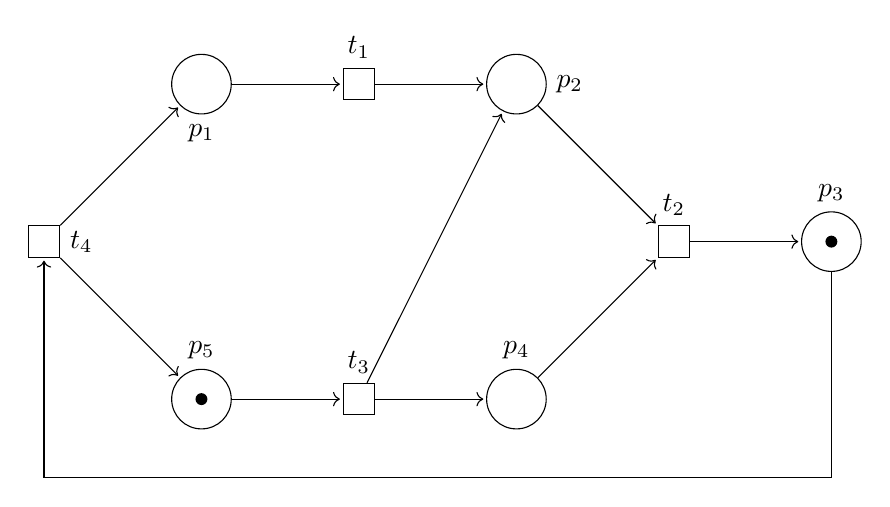
\begin{tikzpicture}
\node[place,tokens=0,label=south:$p_1$] at (2,4) (p1) {};
\node[place,tokens=0,label=east:$p_2$] at (6,4) (p2) {};
\node[place,tokens=1,label=$p_3$] at (10,2) (p3) {};
\node[place,tokens=0,label=$p_4$] at (6,0) (p4) {};
\node[place,tokens=1,label=$p_5$] at (2,0) (p5) {};

\node[transition,label=$t_1$] at (4,4) {}
  edge[pre] (p1)
  edge[post] (p2);
\node[transition,label=$t_2$] at (8,2) {}
  edge[pre] (p2)
  edge[pre] (p4)
  edge[post] (p3);
\node[transition,label=$t_3$] at (4,0) {}
  edge[pre] (p5)
  edge[post] (p2)
  edge[post] (p4);
\node[transition,label=east:$t_4$] at (0,2) (t4) {}
  edge[post] (p1)
  edge[post] (p5);

\draw[pre,bend left=75] (t4) -- (0,-1) -- (10,-1) -- (p3);
\end{tikzpicture}
\end{center}
\end{antwort}

%%
% (b)
%%

\item Berechnen Sie mithilfe der Darstellungsmatrix $A$ und zum
Belegungsvektor $v$, die Belegung nach Schaltung von $t_3 \rightarrow t_2
\rightarrow t_4$.

\begin{antwort}
\begin{displaymath}
v_\text{neu} =
v +
A \cdot \left(\begin{array}{c}0\\0\\1\\0\end{array}\right) +
A \cdot \left(\begin{array}{c}0\\1\\0\\0\end{array}\right) +
A \cdot \left(\begin{array}{c}0\\0\\0\\1\end{array}\right) =
\left(\begin{array}{c}1\\0\\1\\0\\1\end{array}\right)
\end{displaymath}
\end{antwort}

\end{enumerate}

\section{Aufgabe 4: Erreichbarkeitsgraph\footcite[Seite 3]{sosy:ab:4}}

Gegeben ist das folgende Petri-Netz:

\begin{center}
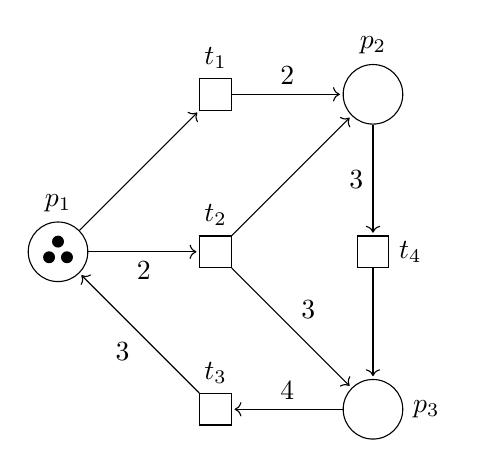
\begin{tikzpicture}
\node[place,tokens=3,label=$p_1$] at (0,2) (p1) {};
\node[place,label=$p_2$] at (4,4) (p2) {};
\node[place,label=east:$p_3$] at (4,0) (p3) {};

\node[transition,label=$t_1$] at (2,4) {}
  edge[pre] (p1)
  edge[post] node[auto]{2} (p2);
\node[transition,label=$t_2$] at (2,2) {}
  edge[pre] node[auto]{2} (p1)
  edge[post] (p2)
  edge[post] node[auto]{3} (p3);
\node[transition,label=$t_3$] at (2,0) {}
  edge[pre] node[auto]{4} (p3)
  edge[post] node[auto]{3} (p1);
\node[transition,label=east:$t_4$] at (4,2) {}
  edge[pre] node[auto]{3} (p2)
  edge[post] (p3);
\end{tikzpicture}
\end{center}

\begin{enumerate}

%%
% (a)
%%

\item Geben Sie die dazugehörige Darstellungsmatrix sowie den
Belegungsvektor an.

\begin{antwort}
\begin{displaymath}
A =
\begin{blockarray}{ccccc}
      & t_1 & t_2 & t_3 & t_4 \\
  \begin{block}{c(cccc)}
  p_1 & -1  & -2  & 3   & 0 \\
  p_2 & 2   & 1   & 0   & -3 \\
  p_3 & 0   & 3   & -4  & 1 \\
  \end{block}
\end{blockarray}
\enspace
,
\enspace
v =
\left(
  \begin{array}{c}
  3 \\
  0 \\
  0
  \end{array}
\right)
\end{displaymath}
\end{antwort}

%%
% (b)
%%

\item Skizzieren Sie den Erreichbarkeitsgraphen des Petri-Netzes.

\begin{antwort}

\end{antwort}

%%
% (c)
%%

\item Begründen Sie anhand des Erreichbarkeitsgraphen, ob das Petri-Netz
verklemmungsfrei ist oder nicht.

\begin{antwort}

\end{antwort}
\end{enumerate}

%-----------------------------------------------------------------------
%
%-----------------------------------------------------------------------

\section{Aufgabe 5 (Check-Up)\footcite[Seite 3]{sosy:ab:4}}
% korrigiert 8.9.2020

Gegeben Sei das folgende Petri-Netz:

\def\TmpCheckup#1{
  \TmpSetKeys%
  \pgfkeys{/petri/.cd,#1}%
  \begin{tikzpicture}
  \node at (-0.25,-0.25) {};
  \node at (\TmpX,\TmpY) {};

  \begin{scope}[transform canvas={scale=\TmpScale},x=1cm,y=1cm,]
    \node[place,tokens=\TmpPlaceOne,label=$p_1$] at (0,3) (p1) {};
    \node[place,tokens=\TmpPlaceTwo,label=$p_2$] at (6,3) (p2) {};
    \node[place,tokens=\TmpPlaceThree,label=south:$p_3$] at (3,0) (p3) {};

    \node[transition,\TmpTransitionOne] at (1.5,1.5) {$t_1$} edge[pre] (p3) edge[post] (p1);
    \node[transition,\TmpTransitionTwo] at (3,3) {$t_2$} edge[pre] (p1) edge[pre] (p2) edge[post] node[auto]{2} (p3);
    \node[transition,\TmpTransitionThree] at (4.5,1.5) {$t_3$} edge[pre] (p3) edge[post] (p2);
    \node[transition,\TmpTransitionFour] at (6,0) {$t_4$} edge[pre] (p2) edge[post] (p3);
    \node[transition,\TmpTransitionFive] at (0,0) {$t_5$} edge[pre] (p1) edge[post] (p3);
  \end{scope}
  \end{tikzpicture}
}

\begin{center}
\TmpCheckup{x=6.4,y=4,scale=1,p3=2}
\end{center}

\begin{enumerate}

%%
% (a)
%%

\item Zeichnen Sie den Erreichbarkeitsgraphen des Petri-Netzes.

\begin{antwort}
\begin{multicols}{2}
\setlength{\parindent}{0cm}
(0,0,2):

\TmpCheckup{x=3.2,y=2,scale=0.5,p3=2,t1,t3}

(1,0,1):

\TmpCheckup{x=3.2,y=2,scale=0.5,p1=1,p3=1,t1,t3,t5}

(0,1,1):

\TmpCheckup{x=3.2,y=2,scale=0.5,p1=0,p2=1,p3=1,t1,t3,t4}

(1,1,0):

\TmpCheckup{x=3.2,y=2,scale=0.5,p1=1,p2=1,p3=0,t2,t4,t5}
\end{multicols}

\begin{center}
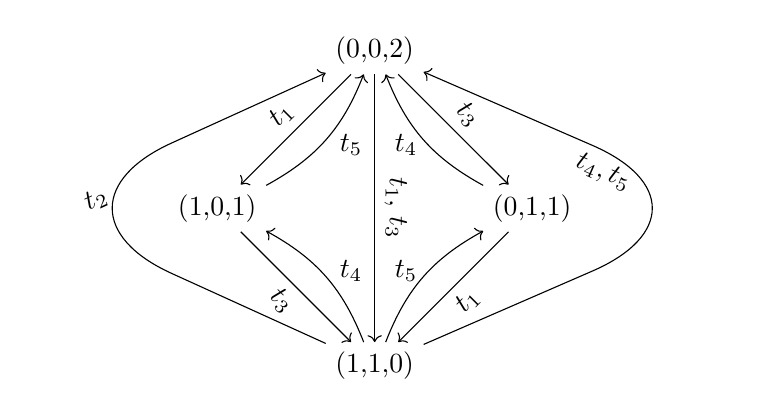
\begin{tikzpicture}[x=2cm,y=2cm]
\def\pfeil#1#2#3#4{\draw[->] (#1) -- (#2) node[pos=0.5,auto,sloped,#4]{#3};}
\node at (2,3) (002) {(0,0,2)};
\node at (1,2) (101) {(1,0,1)};
\node at (3,2) (011) {(0,1,1)};
\node at (2,1) (110) {(1,1,0)};

\pfeil{002}{110}{$t_1$, $t_3$}{}

\draw[->,rounded corners=2cm] (110) -- (-0.2,2) -- (002) node[pos=0.2,sloped,auto,swap]{$t_2$};
\draw[->,rounded corners=2cm] (110) -- (4.3,2) -- (002) node[pos=0.4,sloped,auto,swap]{$t_4,t_5$};

% 002 <-> 011
\pfeil{002}{011}{$t_3$}{}
\draw[->] (011) edge[bend left=20] (002); \node at (2.2,2.4) {$t_4$};

% 002 <-> 101
\pfeil{002}{101}{$t_1$}{}
\draw[->] (101) edge[bend right=20] (002); \node at (1.85,2.4) {$t_5$};

% 101 <-> 011
\draw[->] (101) -- node[sloped,auto,swap]{$t_3$} (110);
\draw[->] (110) edge[bend left=20] (011); \node at (2.2,1.6) {$t_5$};

% 011 <-> 110
\draw[->] (011) -- node[sloped,auto,swap]{$t_1$} (110);
\draw[->] (110) edge[bend right=20] (101); \node at (1.85,1.6) {$t_4$};
\end{tikzpicture}
\end{center}
\end{antwort}

%%
% (b)
%%

\item Begründen Sie anhand des Erreichbarkeitsgraphen, ob das Petri-Netz
lebendig, umkehrbar und/oder verklemmungsfrei ist.

\begin{antwort}

\begin{description}
\item[lebenig]
Ja. Es gibt im Erreichbarkeitsgraphen keine Senke, also keinen Zustand,
aus dem man nicht mehr heraus kommt.

\item[umkehrbar]
Im Erreichbarkeitsgraphen kommt man von (0,0,2) auf verschiedenen Wegen
wieder zurück zu (0,0,2). Man kann sich unendlich oft im Graph bewegen.
Die Anfangsmarkierung kann wieder erreicht werden ($t_1
\rightarrow t_3 \rightarrow t_2$ oder $t_1 \rightarrow t_3 \rightarrow
t_5 \rightarrow t_4$).

\item[verklemmungsfrei] Ja. Es gibt im Erreichbarkeitsgraphen keine
Senke, also keinen Zustand, aus dem man nicht mehr herauskommt.
\end{description}
\end{antwort}

%%
% (c)
%%

\item Geben Sie die Darstellungsmatrix $A$ sowie den Belegungsvektor $v$
an und berechnen Sie damit die Belegung nach Schaltung von $t_1
\rightarrow t_3 \rightarrow t_2$.

\begin{antwort}
\begin{displaymath}
A =
\begin{blockarray}{cccccc}
      & t_1 & t_2 & t_3 & t_4 & t_5 \\
  \begin{block}{c(ccccc)}
  p_1 & 1   & -1  & 0   & 0   & -1  \\
  p_2 & 0   & -1  & 1   & -1  & 0   \\
  p_3 & -1  & 2   & -1  & 1   & 1   \\
  \end{block}
\end{blockarray}
\enspace
,
\enspace
v =
\left(
  \begin{array}{c}
  0 \\
  0 \\
  2
  \end{array}
\right)
\end{displaymath}

\begin{displaymath}
v_\text{neu} =
v +
A \cdot \left(\begin{array}{c}1\\0\\0\\0\\0\end{array}\right) +
A \cdot \left(\begin{array}{c}0\\0\\1\\0\\0\end{array}\right) +
A \cdot \left(\begin{array}{c}0\\1\\0\\0\\0\end{array}\right) =
\left(\begin{array}{c}0\\0\\2\end{array}\right) = v
\end{displaymath}
\end{antwort}

\end{enumerate}

\literatur

\end{document}
